%!TEX root = ../thesis.tex
%*******************************************************************************
%****************************** Fourth Chapter **********************************
%*******************************************************************************
\chapter{Implementation}\label{implementation}

% **************************** Define Graphics Path **************************
\ifpdf
    \graphicspath{{Chapter4/Figs/Raster/}{Chapter4/Figs/PDF/}{Chapter4/Figs/}}
\else
    \graphicspath{{Chapter4/Figs/Vector/}{Chapter4/Figs/}}
\fi

The implementation phase of this project serves to transform the theoretical, mathematical models of Section \ref{Modelling} into functional software capable of solving the defined optimisation problem. This phase was performed simultaneously with the mathematical modelling described in Section \ref{Modelling} and, as such, aligned with the ideals of an agile approach to development as outlined in Section \ref{approachtodev}. Only a high-level detail of integration will be provided as Section \ref{Modelling} details the low-level theory.    

\section{Language}
This system is implemented in Java. This was chosen due to multiple reasons. Firstly, the chosen solver, Gurobi, has a well-documented Java API. This means that troubleshooting is much easier and usage of functions is easier to understand due to the extensive documentation. Secondly, applications written in Java are widely supported by existing platforms meaning the program will be much easier to use on different varieties of computers as intended. Lastly, the author's proficiency in Java ensured less time was consumed when learning the Gurobi API.

\section{Prototyping}
During the development of this project, many prototypes were devised. The first prototype implemented the Minimal Spanning Tree approach as described in Section \ref{Minimal Spanning Tree}. This was successful however suffered from the shortcomings of forming Subtours as shown in Figure \ref{fig:subtours}. The following prototype sought to implement the flow-based system described in Section \ref{A Flow-Based System}, this prototype also integrated a GraphStream\footnote{GraphStream is a Java library for the modelling and analysis of dynamic graphs. \citep{graphstream}} GUI for testing purposes as the previous prototype utilised simple terminal output. The subsequent prototype expanded further upon this GUI, integrating a live callback that displayed the optimiser's current best solution; as opposed to having to having to wait for the optimiser to complete its calculations before outputting a result as was the case with previous prototypes.\newline
The final prototype, before the final application was developed, sought to introduce the Cartesian Grid as described in Section \ref{Cartesian Grid}. This was also successful and as such the proof-of-concept\footnote{Evidence (usually deriving from an experiment or pilot project) demonstrating that a design concept, business idea, etc., is feasible; \citep{oxforduniversitypress_2023_proof}.} is a success. The shortcomings of these prototypes is the method of input for sources and buildings. Within the prototypes, the only way to input data is manually through code. As such this will be addressed in the final application, in order to make it as user-friendly as possible and meet the requirements outlined in Section \ref{systemrequirements}.

\section{Classes}\label{classes}
The classes defined in this section enable the core functionality of the program. In alignment with Object-Oriented Programming (OOP) principles, these classes "seek to model the world by identifying the classes and objects that form the [...] problem" \citep{oop_analysis_with_applications}.

\subsection{Coordinate}
The Coordinate class is defined to store a Node's location in the grid-space. This is a simple $x$ and $y$ integer in a single class alongside a helper function to compare coordinates to allow the application to check if the given coordinates are equal.
\begin{figure}[H]
    \centering
    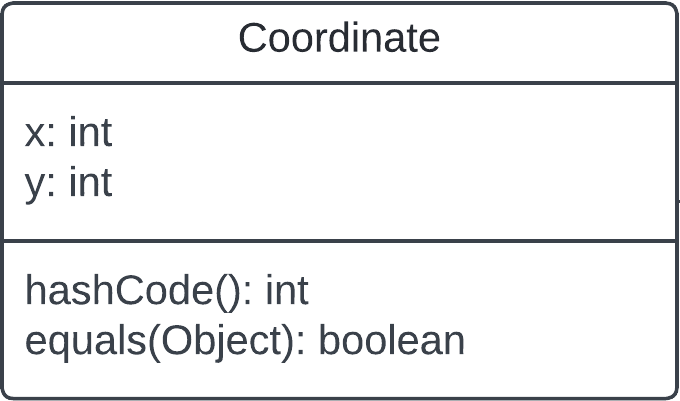
\includegraphics[width=0.3\linewidth]{coordinate_diagram.png}
    \caption{UML Diagram of the Coordinate Class}
    \label{fig:coordinate_uml}
\end{figure}

\subsection{NodeType}
The NodeType class is an enumeration that stores all the potential types of Node that can exist. In this case, a node can be a Building, a Source, or a Junction.
\begin{figure}[H]
    \centering
    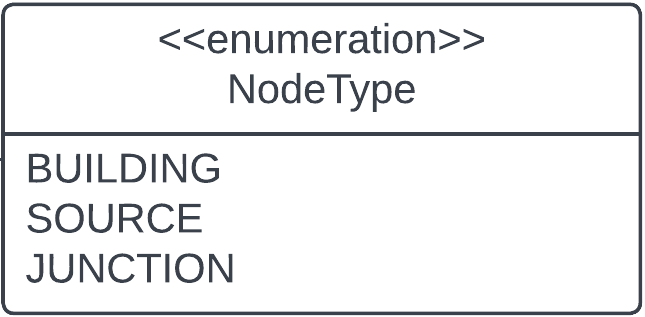
\includegraphics[width=0.3\linewidth]{nodetype_diagram.png}
    \caption{UML Diagram of the NodeType Class}
    \label{fig:nodetype_uml}
\end{figure}

\subsection{Node}
The Node class stores all the potential data a node can require. This include the NodeType, the coordinates, the ID, and the associated pressure information.
\begin{figure}[H]
    \centering
    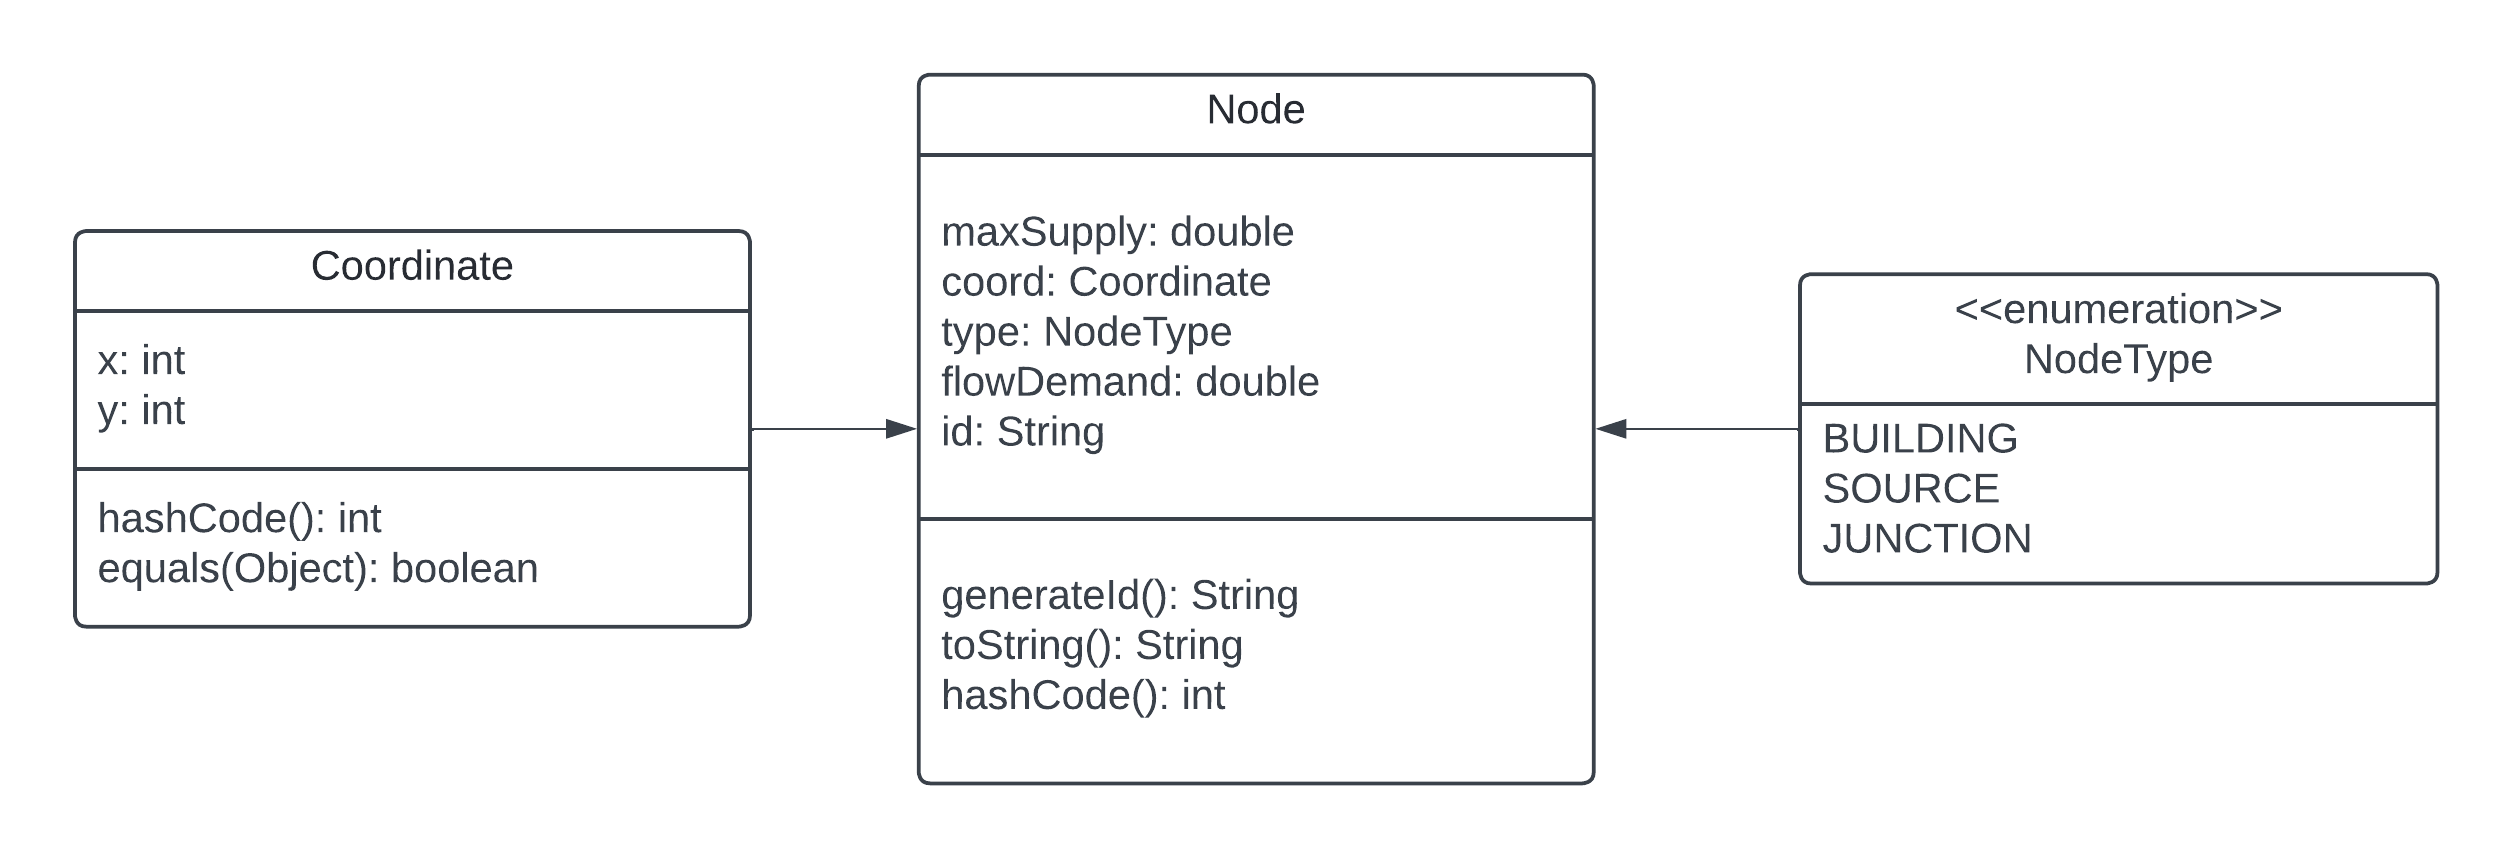
\includegraphics[width=1\linewidth]{Blank diagram (1).png}
    \caption{UML Diagram of the Node Class}
    \label{fig:node_uml}
\end{figure}
The variable $\text{maxSupply}$ is utilised by Source nodes to store their maximum possible pressure output. The variable $\text{flowDemand}$ is utilised by Building nodes to store their water pressure demand.\footnote{The two variables can potentially be contained in a single variable, as they are never both used simultaneously, and should be considered in future work for memory-efficiency.}

\section{Graphical User Interface}\label{gui}
The Graphical User Interface (GUI) front-end was implemented using the Java Swing Library. The primary reason the shift was made from GraphStream in the prototypes, as mentioned earlier, was to enable user inputs. As such, there are several options for the user to interact with.

\begin{figure}[H]
    \centering
    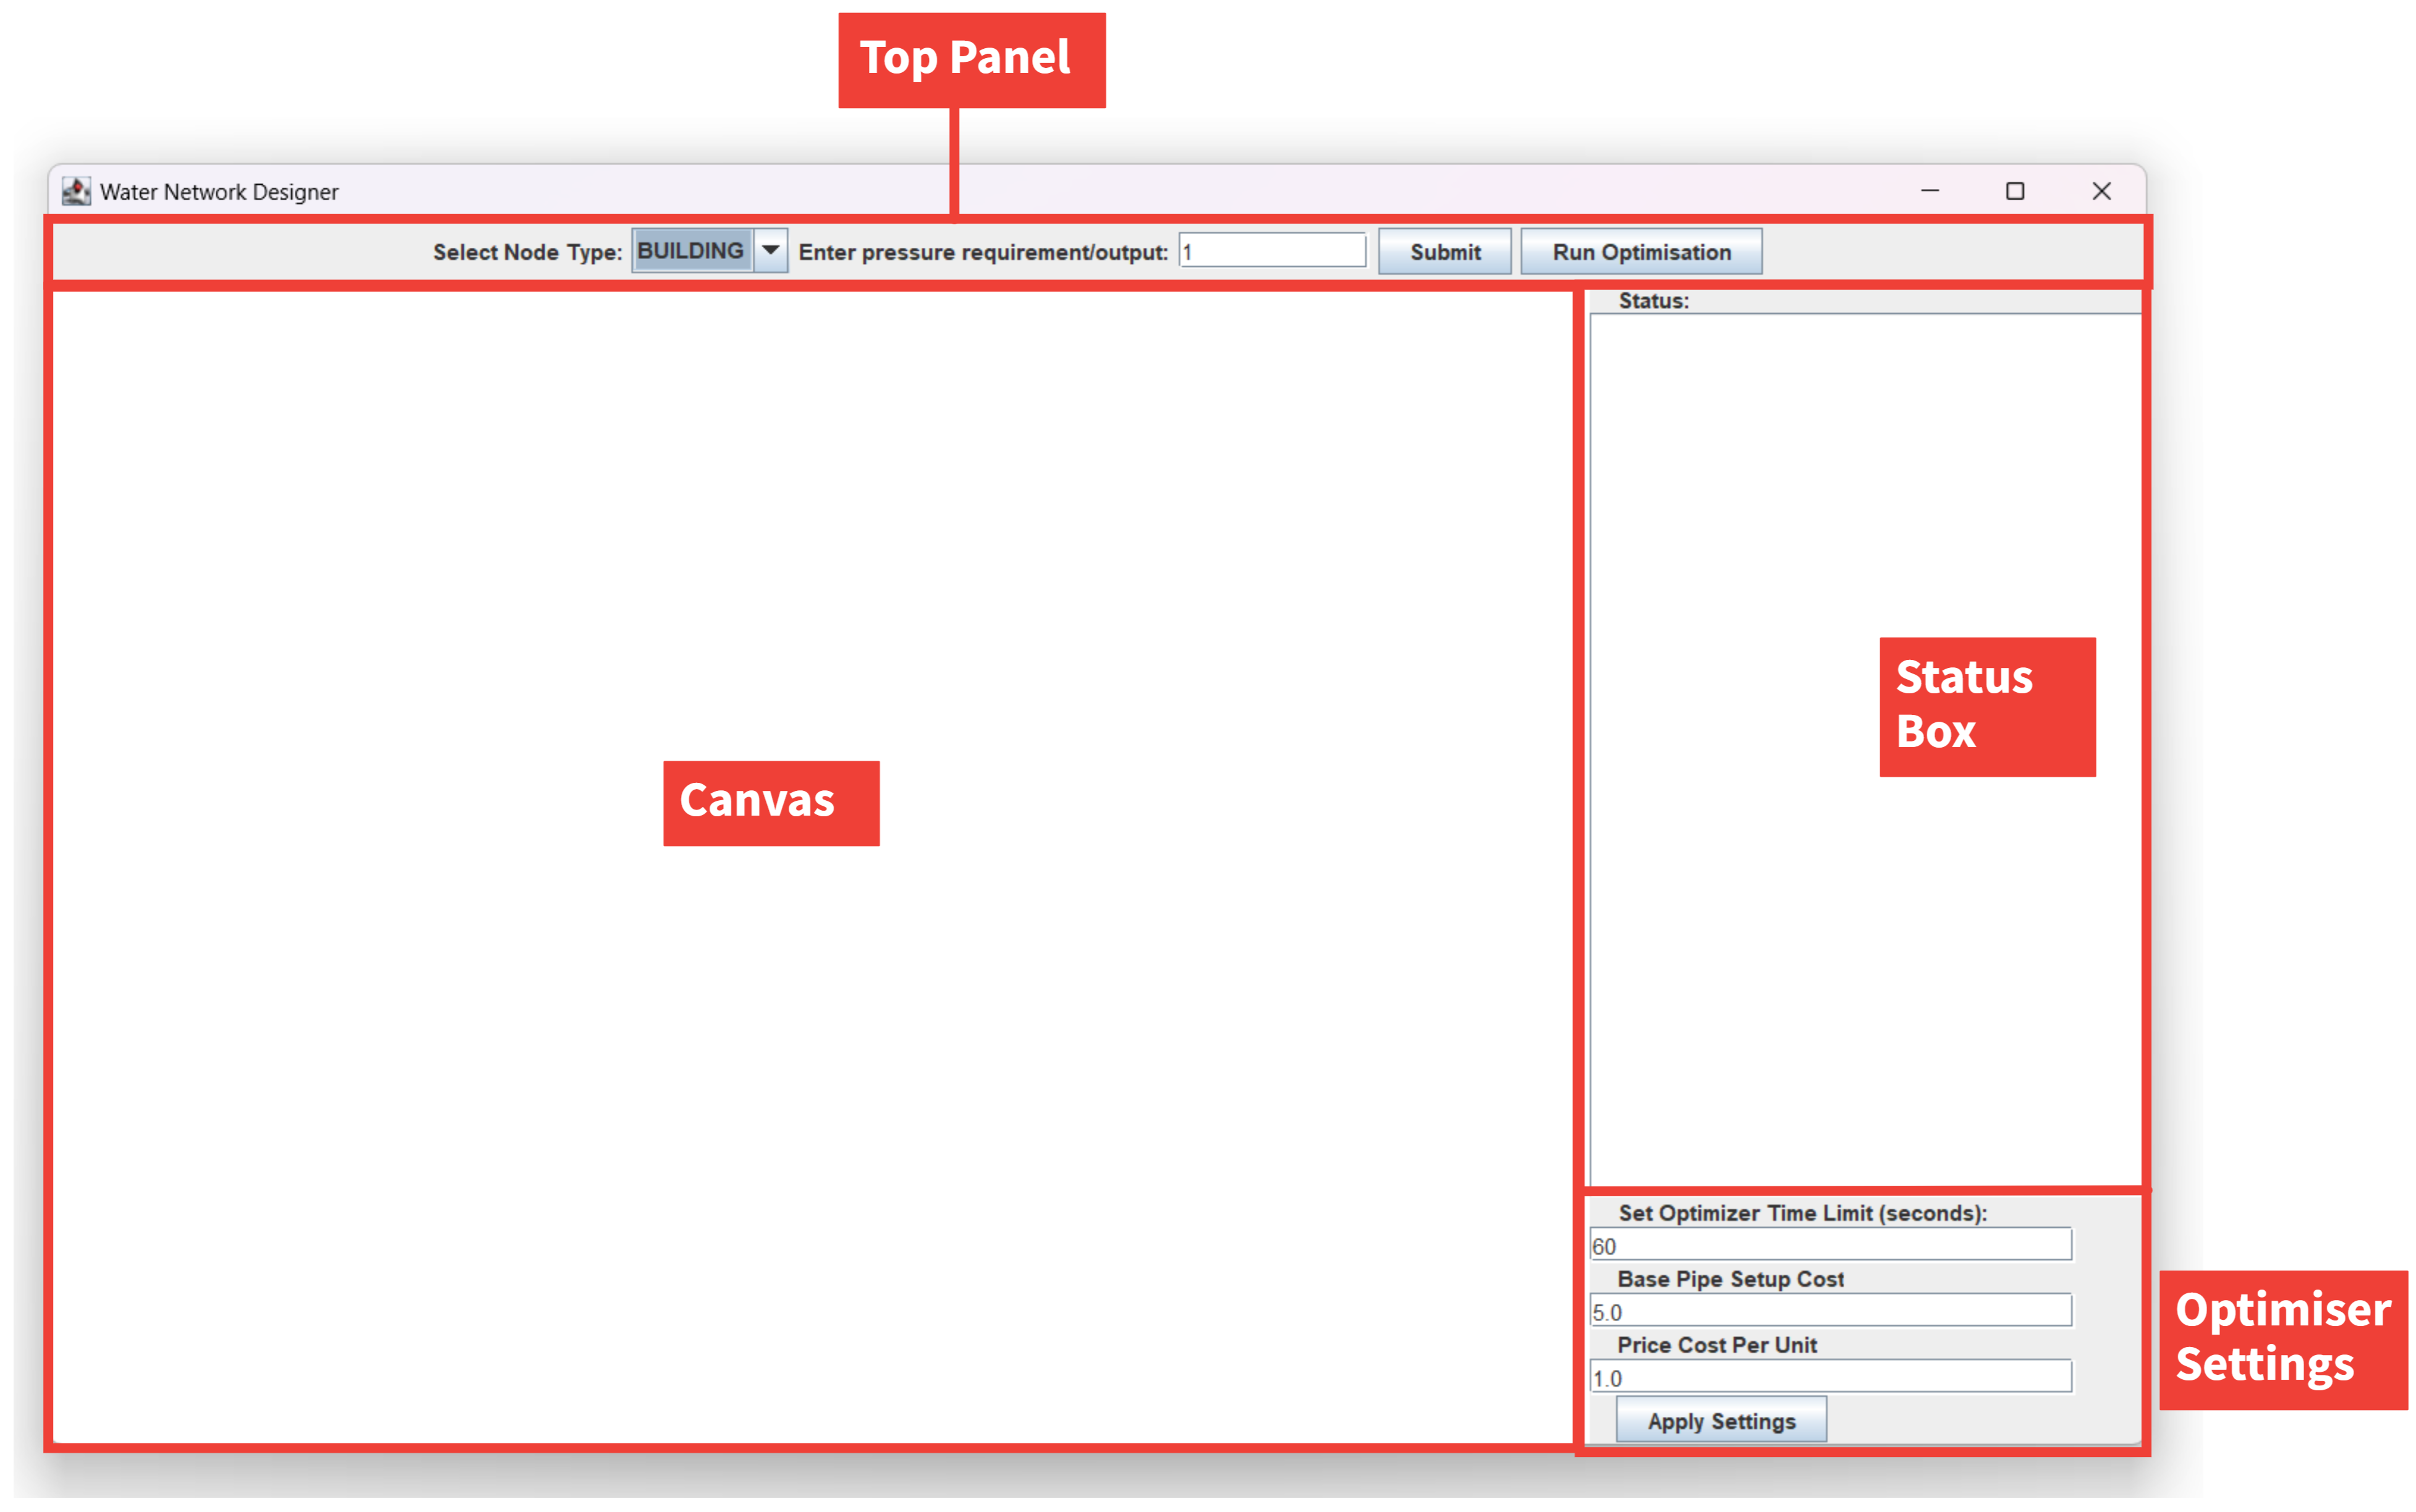
\includegraphics[width=1.0\linewidth]{guimarkup.png}
    \caption{Water Network Designer GUI}
    \label{fig:guimarkup}
\end{figure}


\subsection{Canvas}
The first feature for implementation, and the primary reason for the shift towards a Swing GUI from a GraphStream GUI, was a canvas upon which the user can place nodes. This is highlighted in Figure \ref{fig:guimarkup}. The user simply clicks where they wish to place a node. When this is done, the node is visualised on the canvas and a corresponding status message is displayed as shown in Figure \ref{fig:statusareawithmessages}. 
Buildings are displayed in red and sources are displayed in green as displayed in Figure \ref{fig:canvaswithnodes}.
\begin{figure}[H]
    \centering
    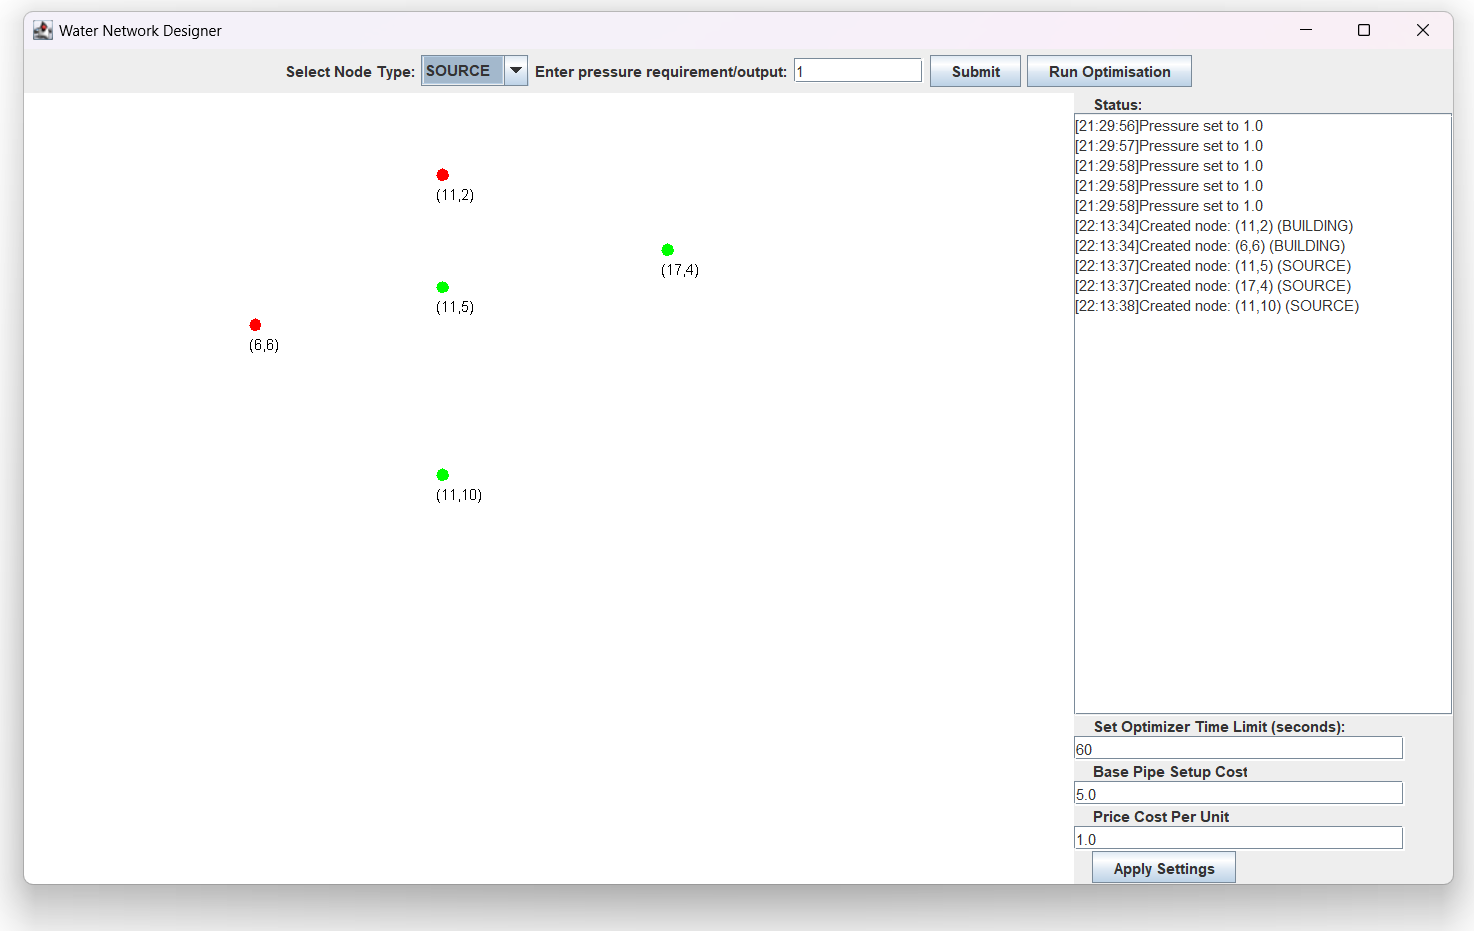
\includegraphics[width=1.0\linewidth]{canvaswithnodes.png}
    \caption{Canvas with Nodes Inputted}
    \label{fig:canvaswithnodes}
\end{figure}

\subsection{Right Panel}
The right panel contains the system settings the user can alter and the system information outputted by the program.

\subsubsection{Status Messages}
Status messages are outputted in the status box as highlighted in Figure \ref{fig:guimarkup} and Figure \ref{fig:statusareawithmessages}.

\paragraph{appendStatus}
Outputting messages to the status area is performed using the helper function appendStatus. This function timestamps all messages, making it easy to track messages as they are outputted. The implementation of this function is contained in Appendix \ref{app:appendStatus}.

\begin{figure}[H]
    \centering
    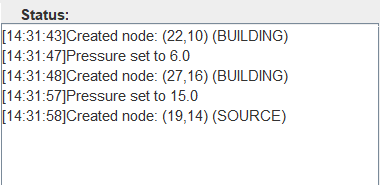
\includegraphics[width=0.5\linewidth]{statusareacloseup.png}
    \caption{Status Box with Time-Stamped Messages}
    \label{fig:statusareawithmessages}
\end{figure}

\subsubsection{System Settings}
This panel also contains the option for the user to alter optimiser parameters. These parameters are as follows:

\begin{longtable}{l p{9cm}}
\caption{Alterable Parameters in the Right Panel}\label{table:alterableparameters} \\
\toprule
Parameter & Description \\
\midrule
\endfirsthead

\multicolumn{2}{c}{{\bfseries \tablename\ \thetable{} -- continued from previous page}} \\
\toprule
Parameter & Description \\
\midrule
\endhead

\midrule \multicolumn{2}{r}{{Continued on next page}} \\
\endfoot

\bottomrule
\endlastfoot

Optimiser Time Limit (seconds) & This parameter alters how long the optimiser runs before terminating.\\
Base Pipe Setup Cost & This parameter defines the minimum cost to setup a pipe. This is the "base" cost before the cost per unit distance.\\
Pipe Cost per Unit & This parameter defines the cost per unit distance of a pipe.\\
\end{longtable}

The user can input these settings in the corresponding text boxes, highlighted in Figure \ref{fig:guimarkup}. To confirm these settings, the user is required to press the apply settings button.

In the event of an invalid input from the user, a corresponding error will appear in a pop-up window and no changes will be made to the settings.
\begin{figure}[H]
    \centering
    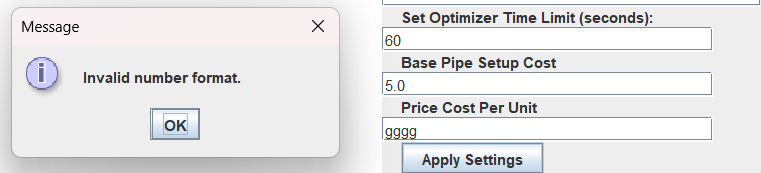
\includegraphics[width=0.6\linewidth]{optimisersettingserror.png}
    \caption{Optimiser Settings Error}
    \label{fig:optimisersettingserror}
\end{figure}

\subsection{Top Panel}
\subsubsection{Node Selection}
To select the type of Node being placed, the user can interact with the drop-down at the top of the GUI. The user can opt to choose between placing Building Nodes and Source Nodes.

\begin{figure}[H]
    \centering
    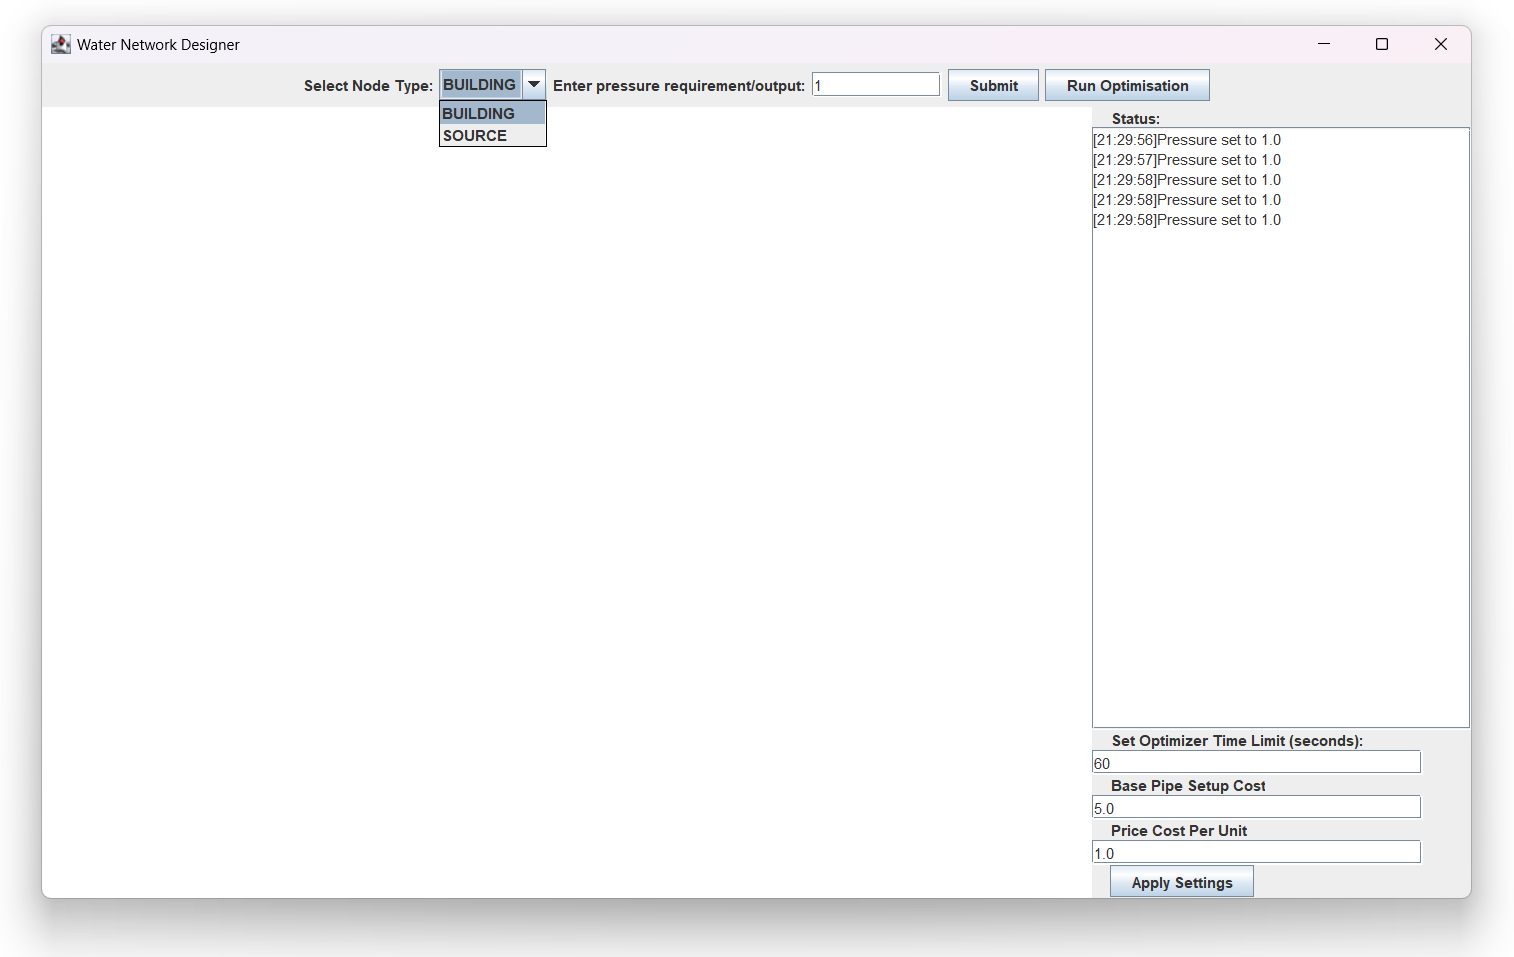
\includegraphics[width=0.8\linewidth]{canvaswithdropdown.png}
    \caption{Canvas with drop-down displayed}
    \label{fig:canvaswithdropdown}
\end{figure}

\subsubsection{Pressure Input}
As displayed in Figure \ref{fig:guimarkup}: from the top panel, the user can also input a pressure variable for the node being placed. To submit the inputted variable, the user is required to press the submit button. When a valid input is submitted a corresponding message is outputted in the Status Area as displayed in Figure \ref{fig:statusareawithmessages}. If input is invalid i.e. not a number, the user is informed through a pop-up window.

\begin{figure}[H]
    \centering
    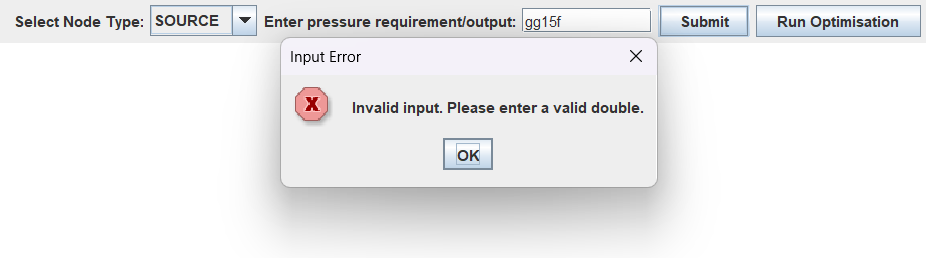
\includegraphics[width=0.8\linewidth]{pressureerror.png}
    \caption{Pressure Input Error}
    \label{fig:pressureerror}
\end{figure}


\subsubsection{Executing Optimisation}
Once the desired nodes are placed on the canvas, the user can execute the optimisation with the \textit{Run Optimisation} button located along the top panel as shown in Figure \ref{fig:guimarkup}.

Upon execution, the junction nodes are calculated and displayed on the GUI as well as the optimal piping route currently calculated.
\begin{figure}[H]
    \centering
    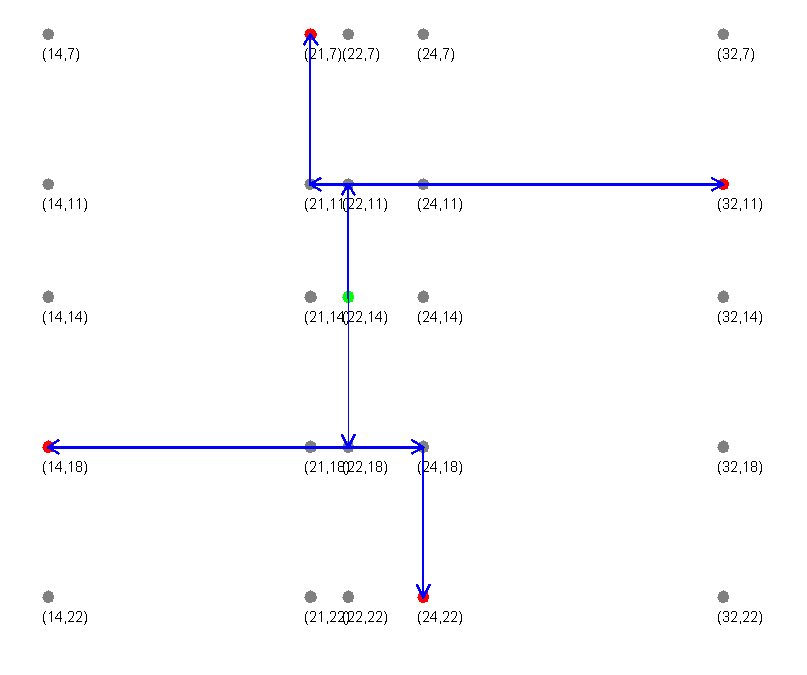
\includegraphics[width=0.7\linewidth]{optimisationexecution.png}
    \caption{Optimisation Execution Example}
    \label{fig:optimisationexecuting}
\end{figure}

The optimiser's progress and messages will be outputted to the status menu.

\begin{figure}[H]
    \centering
    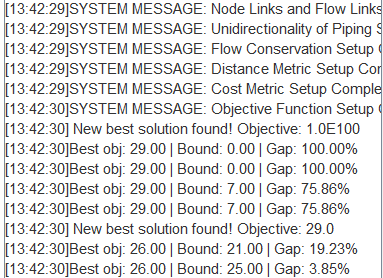
\includegraphics[width=0.5\linewidth]{optimiserprogress.png}
    \caption{Optimiser Status Messages}
    \label{fig:optimiserprogress}
\end{figure}

The user is notified once the optimiser has completed.

\begin{figure}[H]
    \centering
    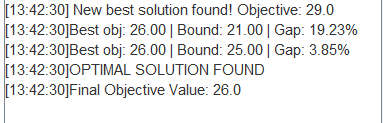
\includegraphics[width=0.5\linewidth]{optimisercompletion.png}
    \caption{Optimiser Completion Messages}
    \label{fig:optimisercompletion}
\end{figure}

In the event the model is infeasible - typically due to the pressure required by buildings being greater than the total pressure available in the system - the user is notified in the status menu.

\begin{figure}[H]
    \centering
    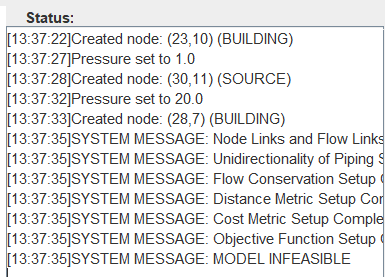
\includegraphics[width=0.5\linewidth]{infeasiblemodelerror.png}
    \caption{Infeasible Model Status Message}
    \label{fig:infeasiblemodelerror}
\end{figure}


\section{Solver}\label{solver}
This section details the implementation of the solver. The optimisation logic is driven by Gurobi, as established in Section \ref{evaluationofsolvers}. Within the context of this project, Gurobi is used to determine the most cost-effective layout of a pipe network, subject to strict structural and physical constraints. These constraints are established in Section \ref{Modelling} and the implementation of which is outlined in Section \ref{constraints}.

\subsection{Application-Solver Interaction}
The Gurobi Optimiser runs as a separate application on the computer to the application being implemented. Interactions between the solver and the application are handled through the API contained in the \textit{gurobi.jar} package. 


\subsection{Importing Data}
Importing all the necessary data to the solver is as expected, as the data is stored in sets and lists and is simply required to be importing into the solver's function when the optimiser is run. These sets and lists are outlined in Figure \ref{fig:setsandlists_uml}.
\begin{figure}[H]
    \centering
    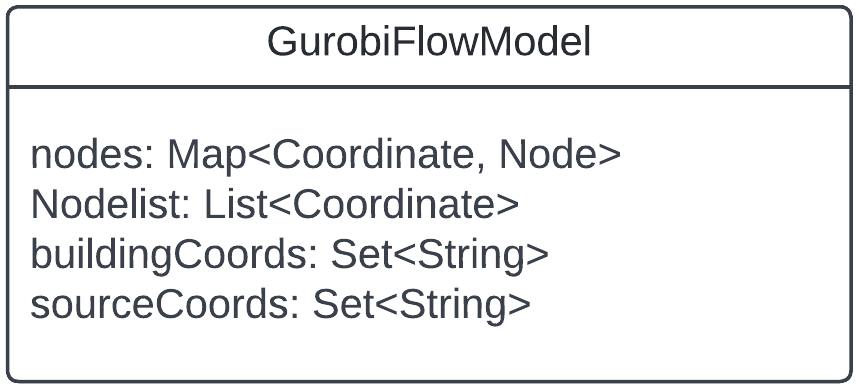
\includegraphics[width=0.4\linewidth]{nodeslistdiagram.png}
    \caption{UML Diagram of the Sets and Lists within the GurobiFlowModel Class}
    \label{fig:setsandlists_uml}
\end{figure}
The HashMap titled "nodes" maps Co-ordinates to Nodes and stores the details of a Node at a given coordinate. Using a HashMap means that only a single Node can exist at a single point as each key for the HashMap - coordinates in this case - can only be used once. The list 'Nodelist' stores each Node object in the model - this means it also contains each Node's corresponding information. The Sets of Strings - 'buildingCoords' and 'sourceCoords' - store the coordinate keys of every Node of that type. These are stored seperately as they are retained for use when generating the Cartesian Grid and when establishing Flow Conservation Laws for each Node.


\subsection{Constraints}\label{constraints}
Each constraint upon the solver establishes a new rule/law the solver must follow when determining a final solution. These constraints also generate Gurobi Variables where appropriate for use in conjunction with the Gurobi Optimiser.

\subsubsection{Node and Flow Links}
This constraint implements the node and flow links. These enforce which node connections can exist and therefore where flow can exist. These variables also store the $n_{ij}$ - connection values - and $f_{ij}$ - the flow between two points. This is covered in detail in Section \ref{nodeandflowlinks}.
\begin{lstlisting}
for (int i = 0; i < N; i++){
    for (int j = 0; j < N; j++){
        if (i != j && areParallel(Nodelist.get(i), Nodelist.get(j))){
            n[i][j] = model.addVar(0, 1, 0, GRB.BINARY, "n_"+i+"_"+j);
            f[i][j] = model.addVar(0, maxFlow, 0, GRB.CONTINUOUS, "f_"+i+"_"+j);
        }
    }
}
\end{lstlisting}

\subsubsection{Flow Can Only Exist upon a connection}
This constraint ensures that flow can only travel over node links that exist. This is covered in detail in Section \ref{flowonexistingedge}.
\begin{lstlisting}
for (int i = 0; i < N; i++){
    for (int j = 0; j < N; j++){
        if (n[i][j] != null){
            GRBLinExpr expr = new GRBLinExpr();
            expr.addTerm(maxFlow, n[i][j]);
            model.addConstr(f[i][j], GRB.LESS_EQUAL, expr, "flow_limit_"+i+"_"+j);
        }
    }
}
\end{lstlisting}

\subsubsection{Uni-Directionality of Piping}
This constraint ensures that if a connection exists, the reverse connection cannot exist as pipes must be uni-directional. This is covered in detail in Section \ref{Breaking Symmetry}.
\begin{lstlisting}
for (int i = 0; i < N; i++){
    for (int j = 0; j < N; j++){
        if (n[i][j] != null && n[j][i] != null){
            GRBLinExpr expr = new GRBLinExpr();
            expr.addTerm(1.0, n[i][j]);
            expr.addTerm(1.0, n[j][i]);

            model.addConstr(expr, GRB.LESS_EQUAL, 1.0, "no_bidirectional_"+i+"_"+j);
        }
    }
}
\end{lstlisting}

\subsubsection{Flow Conservation}
These constraints establish the flow rules for each node, as covered in Sections \ref{flowconservation} and \ref{alteringflowconservation}.
\begin{lstlisting}
for (int x = 0; x < N; x++){
    Node node = nodes.get(Nodelist.get(x));

    GRBLinExpr inflow = new GRBLinExpr();
    GRBLinExpr outflow = new GRBLinExpr();

    for (int i = 0; i < N; i++){
        if (f[i][x] != null) inflow.addTerm(1.0, f[i][x]);
        if (f[x][i] != null) outflow.addTerm(1.0, f[x][i]);
    }

    switch(node.getType()){
        case NodeType.SOURCE:
            model.addConstr(inflow, GRB.EQUAL, 0.0, "src_in_" + x);
            model.addConstr(outflow, GRB.LESS_EQUAL, node.getMaxSupply(), "src_out_" + x);
            break;
        case NodeType.BUILDING:
            // Adjusted constraint: outflow = inflow - pressureRequirement
            GRBLinExpr lhs = new GRBLinExpr();
            lhs.multAdd(1.0, inflow);
            lhs.multAdd(-1.0, outflow);
            model.addConstr(lhs, GRB.EQUAL, node.getFlowDemand(), "bldg_balance_"+x);
            model.addConstr(inflow, GRB.GREATER_EQUAL, node.getFlowDemand(), "bldg_in_"+x);
            break;
        case NodeType.JUNCTION:
            model.addConstr(inflow, GRB.EQUAL, outflow, "junc_" + x);
            break;
    }
}
\end{lstlisting}

\subsubsection{Defining Distance}
This constraint calculates distance to store in $d_{ij}$ as part of the cost function as devised in Section \ref{definingdistance}.
\begin{lstlisting}
Map<String, Double> d = new HashMap<>();
for (int i = 0; i < N; i++){
    for (int j = 0; j < N; j++){
        if (n[i][j] != null){
            String key = nodes.get(Nodelist.get(i)).getId() + "_" + nodes.get(Nodelist.get(j)).getId();
            double dist = calcEuclidDistance(nodes.get(Nodelist.get(i)), nodes.get(Nodelist.get(j)));
            d.put(key, dist);
        }
    }
}
\end{lstlisting}

\subsubsection{Defining Cost}
This constraint defines the cost for a connection as established in Section \ref{definingcost}.
\begin{lstlisting}
double[][] c = new double[N][N];
for (int i = 0; i < N; i++){
    for (int j = 0; j < N; j++){
        if (n[i][j] != null){
            c[i][j] = (d.get(nodes.get(Nodelist.get(i)).getId() + "_" + nodes.get(Nodelist.get(j)).getId()) * costPerUnitPipe) + pipeBaseSetup;
        }
    }
}
\end{lstlisting}

\subsubsection{Objective Function}
This constraint establishes the Objective Function for the optimiser. This is covered in Section \ref{finalobjfunc}.
\begin{lstlisting}
GRBLinExpr obj = new GRBLinExpr();
for (int i = 0; i < N; i++){
    for (int j = 0; j < N; j++){
        if (n[i][j] != null){
            double dist = calcEuclidDistance(nodes.get(Nodelist.get(i)), nodes.get(Nodelist.get(j)));
            obj.addTerm(c[i][j], n[i][j]);
        }
    }
}
model.setObjective(obj, GRB.MINIMIZE);
\end{lstlisting}

\subsection{A Live Callback}
In order to update the GUI \textit{whilst} the optimiser solves the problem - as opposed to waiting for the solver to finish before outputting a solution - it is required to implement a callback. A callback is a direct feature of the Gurobi Framework and enables the live feedback of the current best solution determined by the optimiser. This is implemented by creating a new class, in this case called "LiveCallback", which extends the GRBCallback class. In this case, the callback was utilised for two primary purposes: updating the GUI to show the current best solution, and relaying the same information as a Status Message in the dedicated status area. This was implemented through a list which tracks the current active connections. When a better solution is calculated, the list of active connections is updated and the front-end is updated accordingly. The status area is then updated accordingly also. For a full code snippet see Appendix \ref{app:callback_code}.

\subsection{Determining the Upper Bound of the Flow Constraint}
As established in Section \ref{flowonexistingedge}, it is required to set an upper bound for flow constraints. This is simply referred to as \textit{maxFlow}. A simple solution would be to set this bound to positive infinity as this would satisfy the constraint as any flow value would fall under this value, however, a more optimal solution is to calculate the actual maximum possible flow through all pipes. This can be calculated from the total flow output of every source node in the graph.

\begin{lstlisting}
double maxFlow = 0;
for (Node node : nodes.values()){
    if (node.getType() == NodeType.SOURCE){
        maxFlow = maxFlow + node.getMaxSupply();
    }
}
\end{lstlisting}

\section{Multi-Threading}
In order to ensure adequate performance, and ensure it remains possible to receive intermediate solutions from the optimiser without delaying the optimisers runtime, multi-threading is required. This has been implemented such that the Swing GUI is running in the main thread and the optimisation process is operating in a background thread. This was simply implemented using the \textit{Thread} module from the \textit{java.lang} package.

\section{Outcome}
In this section, the final implementation of the optimisation system is presented, showcasing the functionality and results achieved through the optimisation process. Building upon the earlier outlined design and approach, this section highlights the working prototype.

\subsection{System Specifications}\label{sysinfo}
These simulations were ran on a Framework Laptop 13, fitted with an Intel Core i5-1340p and 16GB of RAM. For full System Specifications see Appendix \ref{app:sysinfo}.

\subsection{Trial}
This trial being ran will contain twenty Building Nodes, each with a pressure requirement of one, and five Source Nodes, each with a pressure of four. Planning this by hand would typically take a significant amount of time, however, to prove the system's capabilities, it will be limited to the best solution found within five minutes. The base setup cost is set to five and the pipe cost per unit is set to one.\newline\newline
The input is available in Figure \ref{fig:testinput} and the output is available in Figure \ref{fig:testoutput}. 
An important note to make is that the system had not yet finished computing after five minutes. However, the best objective value of 344 was determined thirteen seconds into the program's runtime, showcasing it's efficiency. Even given the high amount of information present on the graph, it is still easy to discern different nodes and consume the information.

\begin{landscape}
\begin{figure}[H]
    \centering
    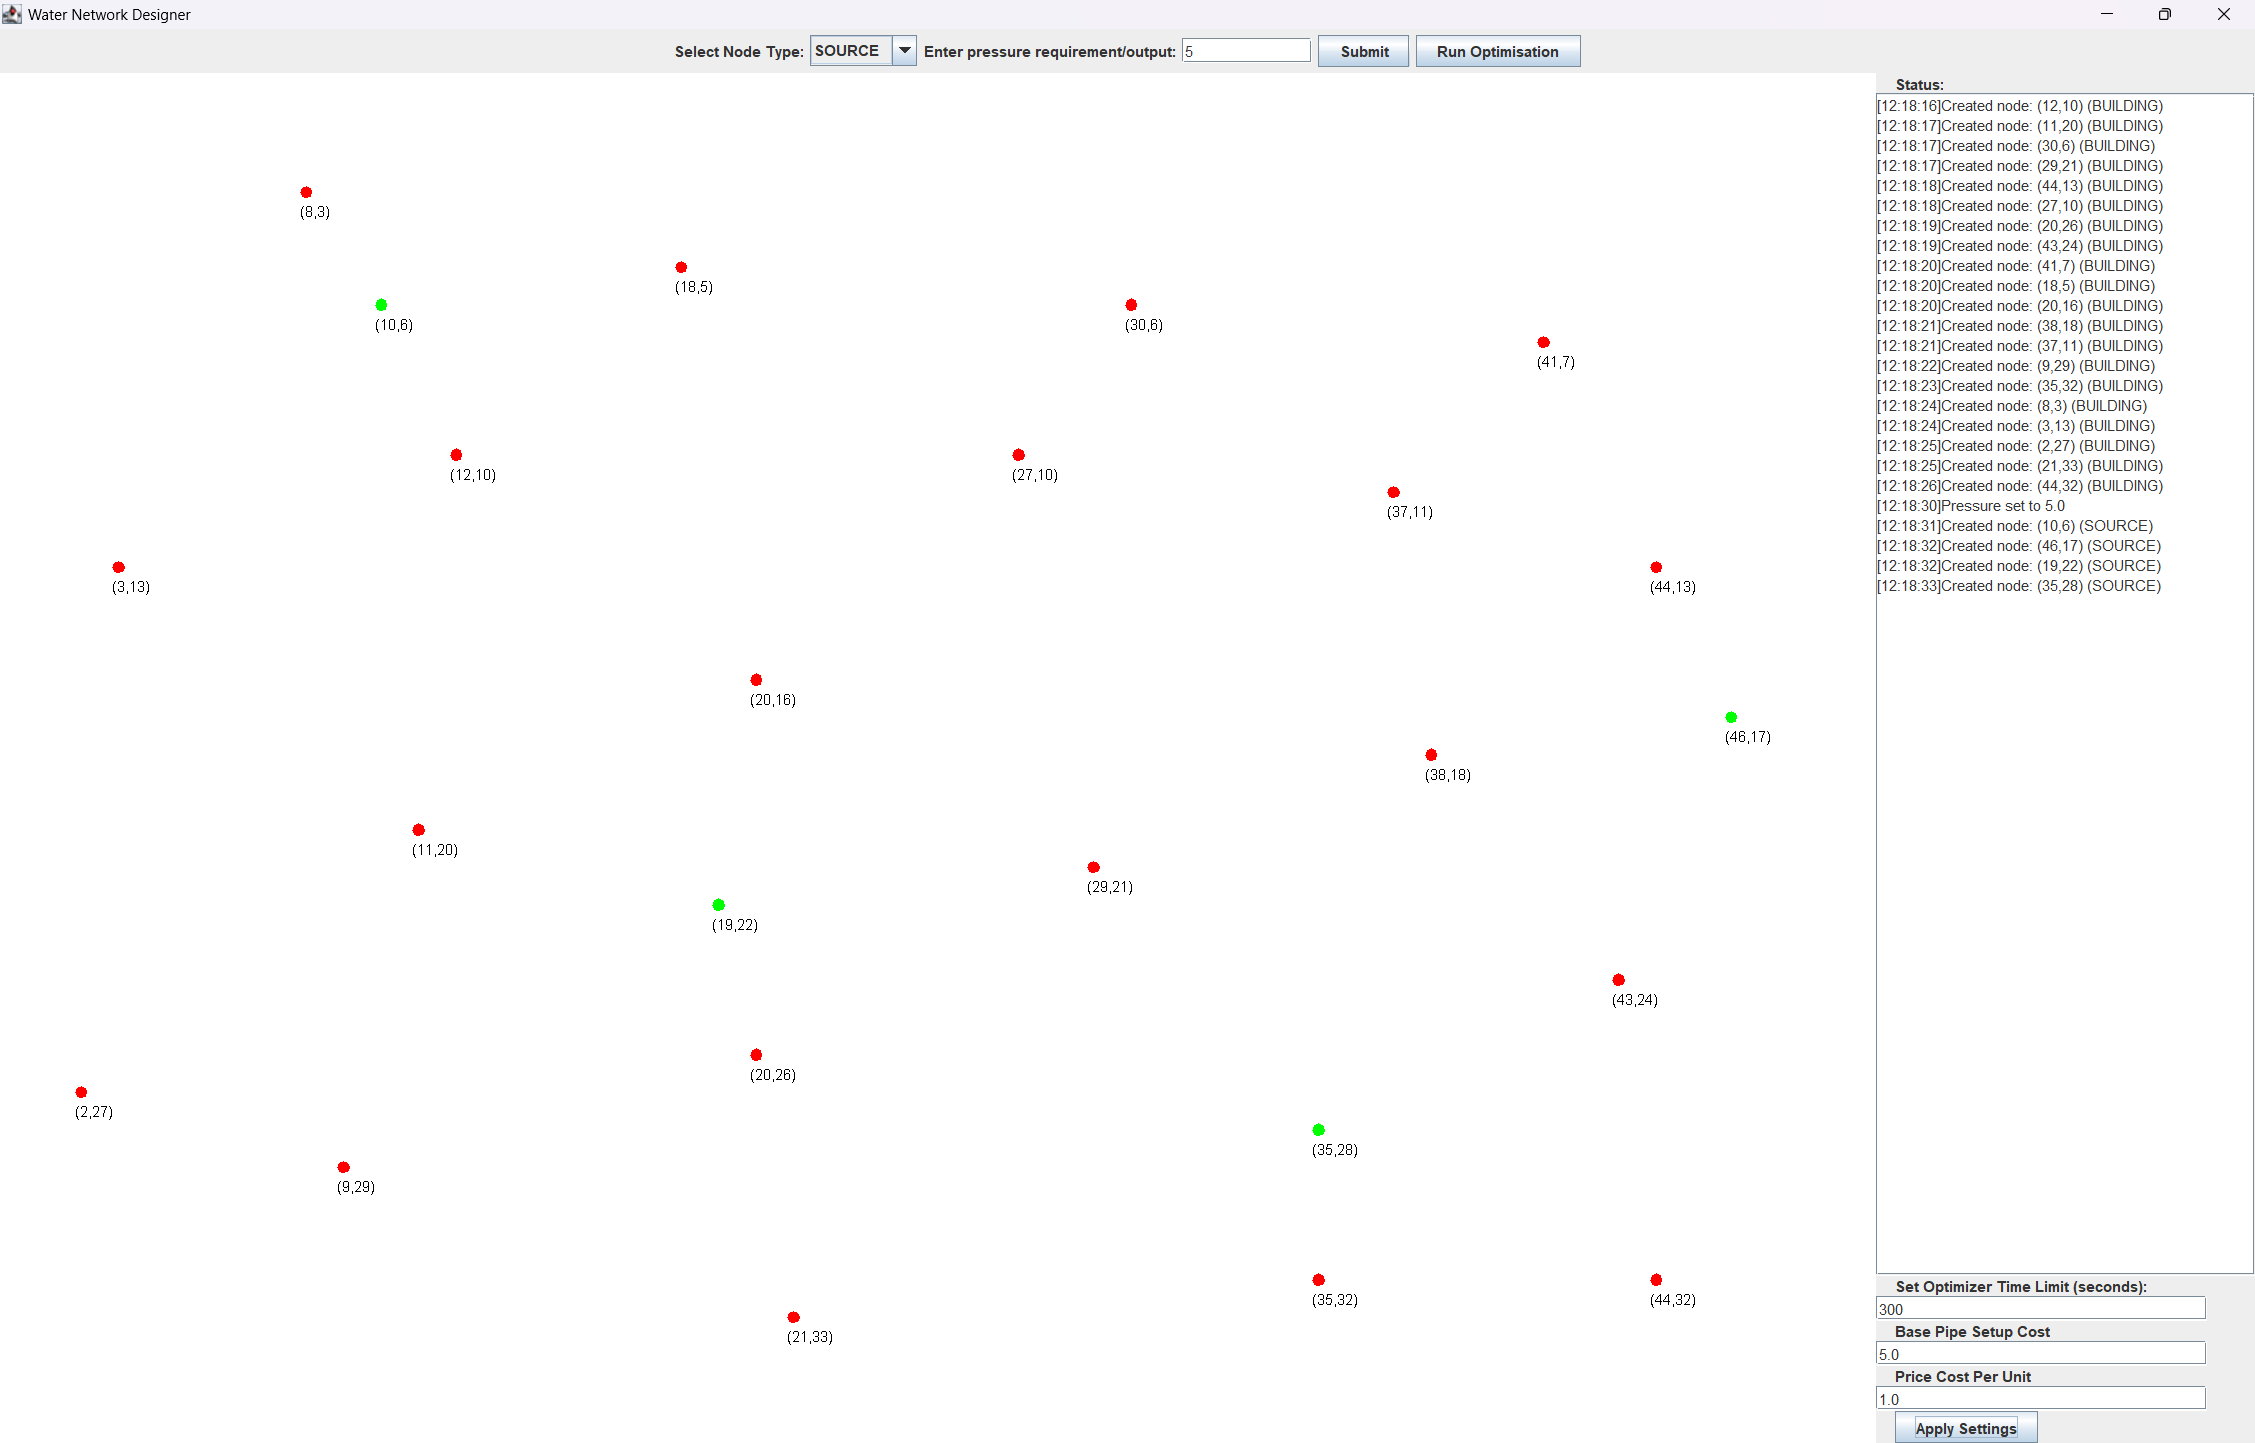
\includegraphics[width=0.9\linewidth]{input.png}
    \caption{Input to the Program}
    \label{fig:testinput}
\end{figure}
\begin{figure}[H]
    \centering
    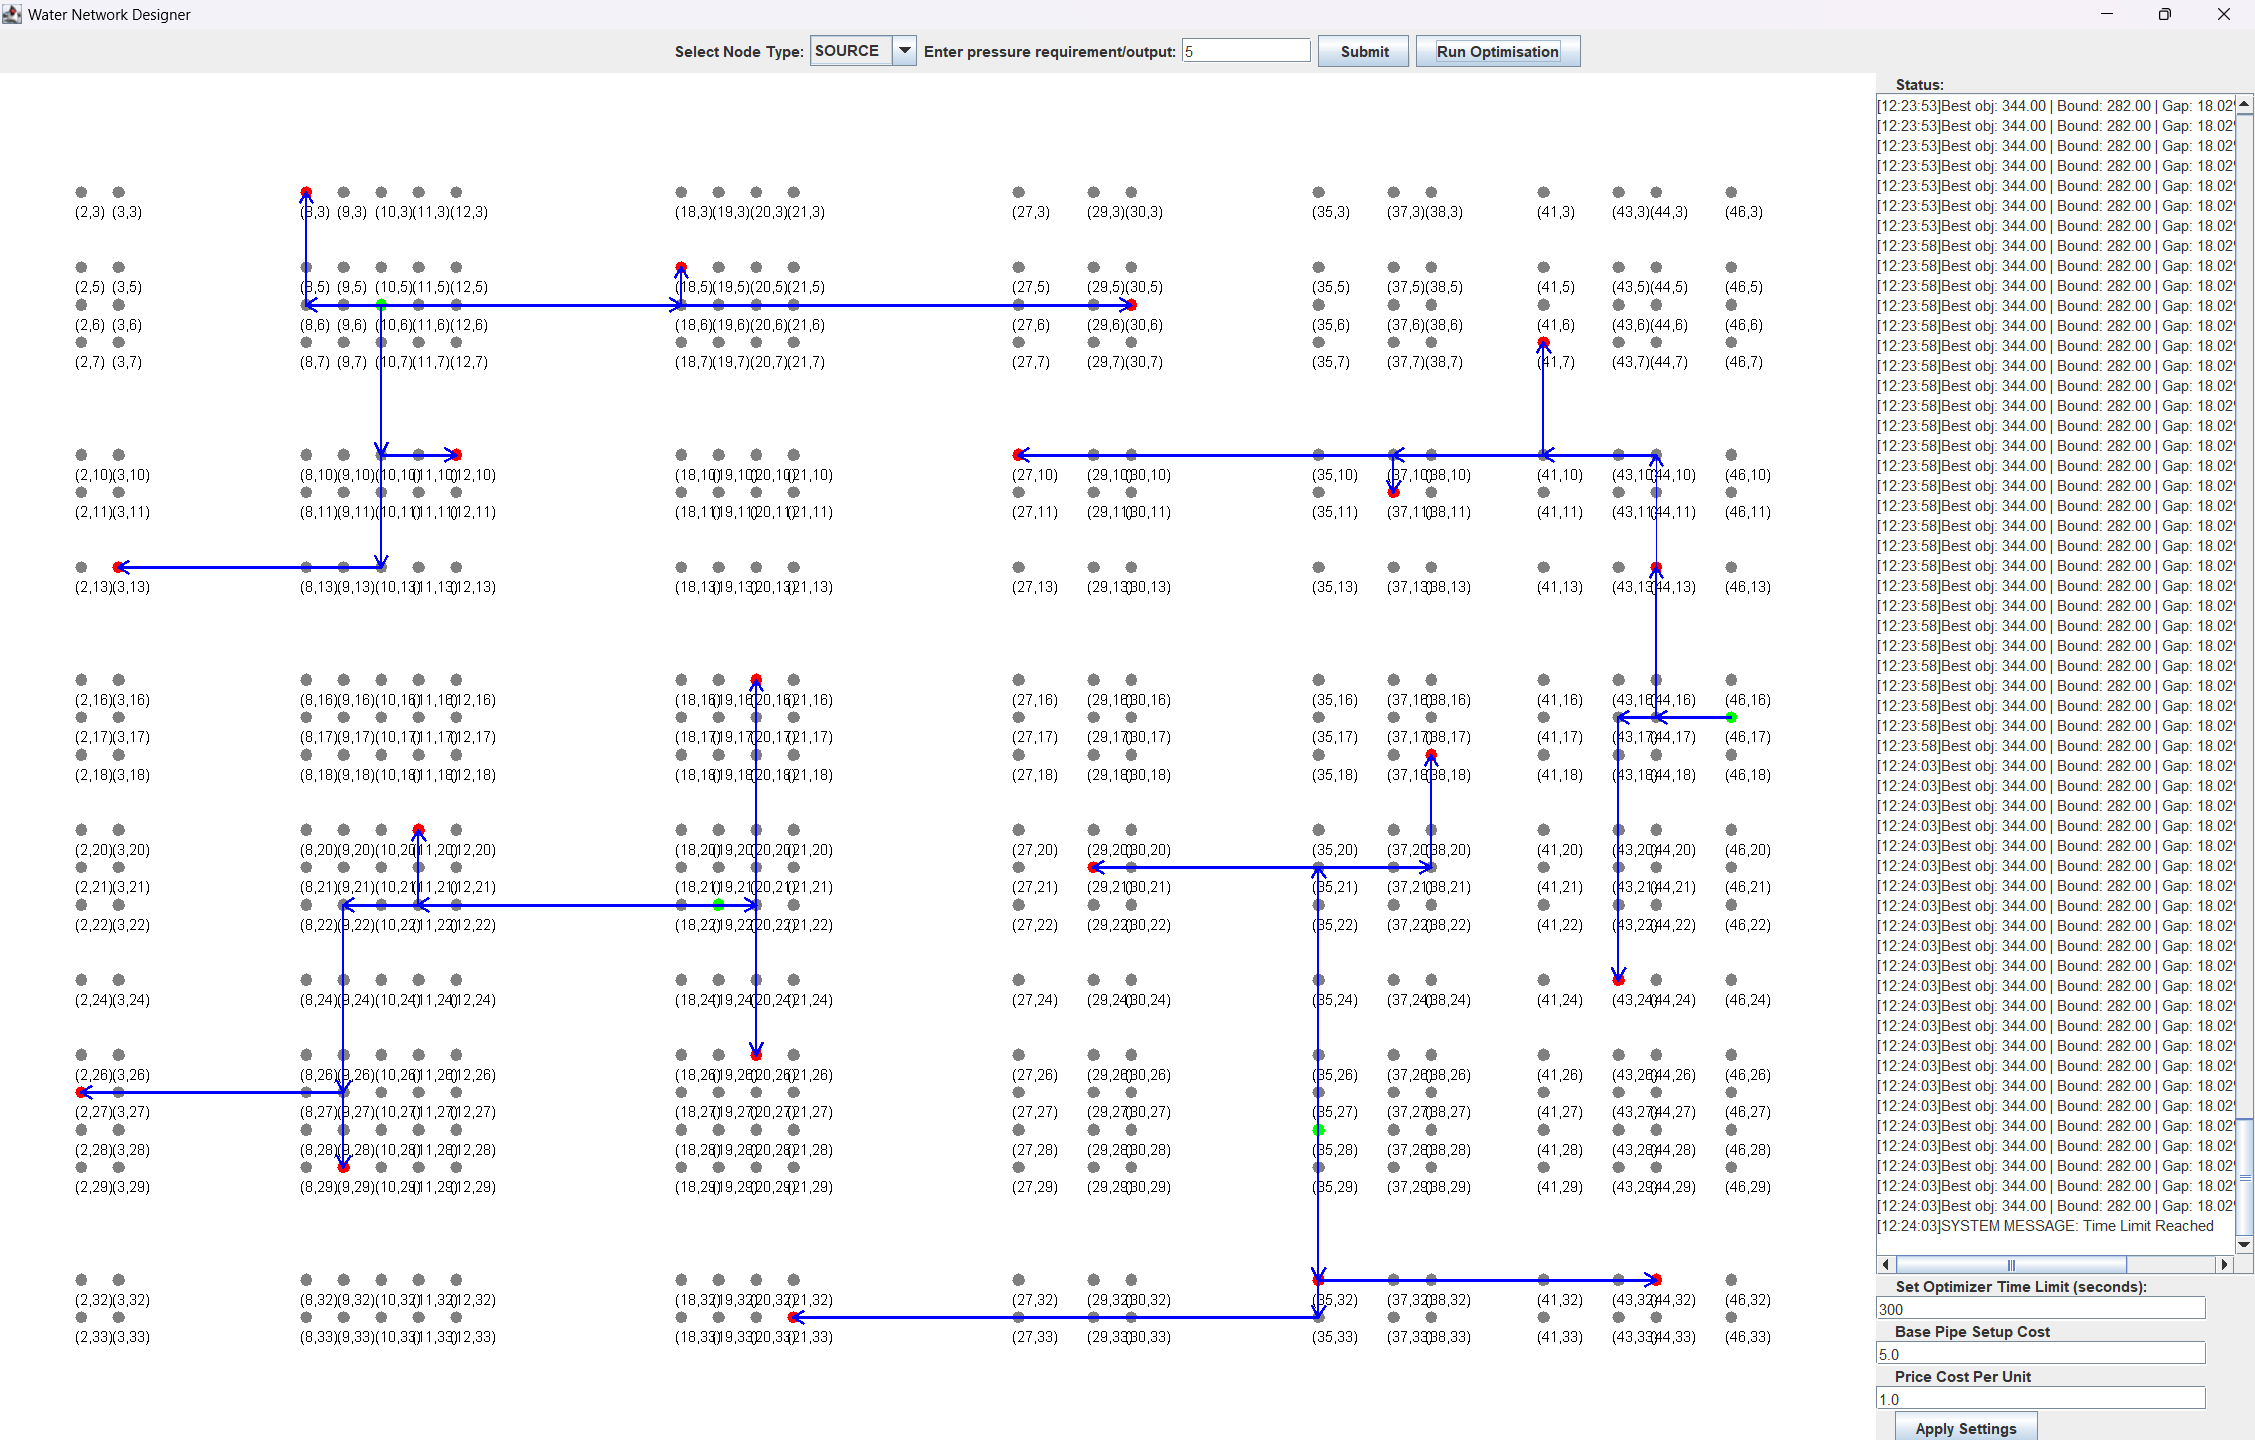
\includegraphics[width=0.9\linewidth]{output.png}
    \caption{Output from the Program}
    \label{fig:testoutput}
\end{figure}
\end{landscape}